% Section content template for individual Educative lessons
% This file contains the actual content for a specific section
% Generated from Educative API section content

% Section: System Design: ChatGPT System
% Section ID: 6392521611411456
% Section Slug: system-design-chatgpt-system
% Generated: 2025-12-08T15:34:59.109077

\subsection{What is ChatGPT?}\label{GcmYZRoJV5NFbJp7IlYPt}
\\
\textbf{ChatGPT} is an advanced conversational application built on a sophisticated artificial intelligence language model developed by OpenAI. It is designed to understand natural language and generate human-like text, making it a highly effective tool for various communication tasks. Clear and effective communication is essential in various situations, including explaining complex concepts, generating ideas, and crafting professional content. In these cases, ChatGPT can help by:

\begin{itemize}
\item
\protect\phantomsection\label{VPLyD2ENnyJowGgz7upA5}
Simplifying technical subjects.
\item
\protect\phantomsection\label{mI-Z6MBvFPv-qQ3oCLbLF}
Proposing innovative ideas.
\item
\protect\phantomsection\label{TV4zOegID4eD4WoAit8kJ}
Composing clear, well-structured text.
\end{itemize}

\begin{figure}[htbp]
 \centering
 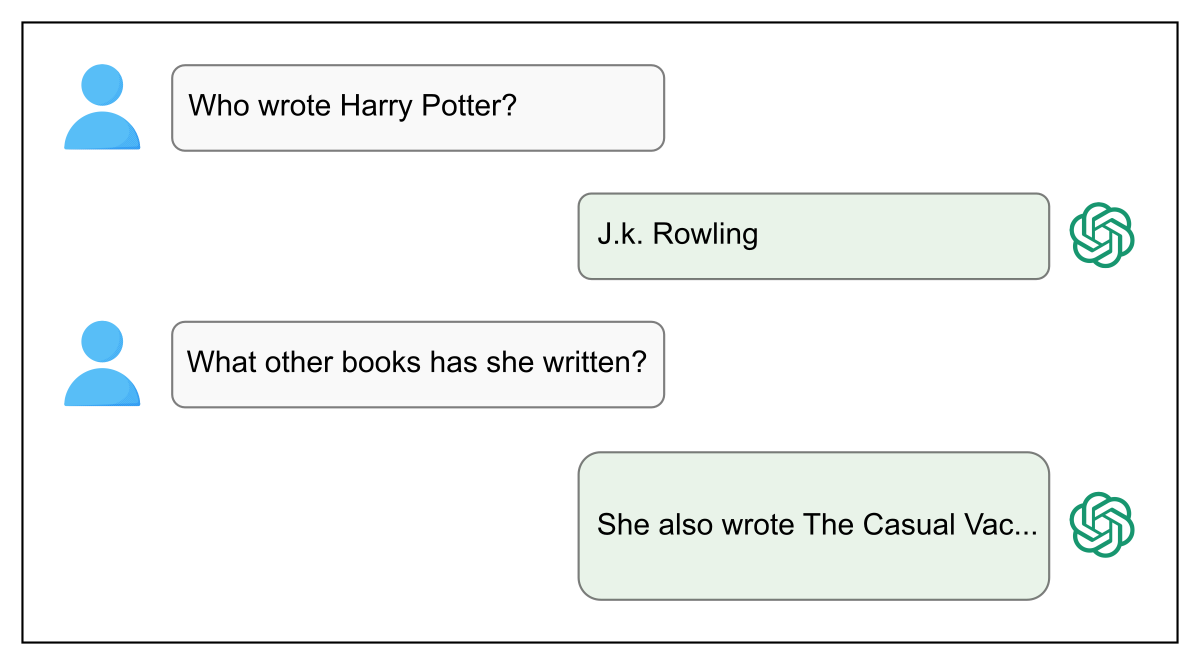
\includegraphics[width=0.5\textwidth]{Images/chapter_41/section_6392521611411456/4829897081880576.png}
 \caption{ChatGPT understands context and provides relevant follow-up responses}
\end{figure}

ChatGPT-like systems are particularly noteworthy because they can interpret various inputs, even when prompts are incomplete or ambiguous. They can respond to complex, abstract, or open-ended questions with clarity and relevance. These capabilities are made possible by sophisticated generative AI techniques, extensive training on large datasets, and advanced language modeling. Rather than relying on predefined answers, such systems analyze context, identify patterns in language, and generate responses that align with the intent and structure of the input.
\\
In this chapter, we'll design a text-to-text generation system similar to ChatGPT. While OpenAI has not publicly disclosed the exact architecture and design details of ChatGPT, the approach covered in this lesson is based on general principles, established techniques, and best practices commonly used in building such systems.\\
\strut \\
Let's start by defining the core requirements, which play a critical role in shaping the overall design:

\subsubsection{Requirements}\label{FZMkX0TR-QmIkF-MWdBVA}
\\
Building the backend of a text-to-text generation system like ChatGPT requires careful attention to both functional and non-functional requirements:
\\
\paragraph{Functional requirements}\label{DFCd17zFOBGViuQafshyy}

\begin{itemize}
\item
\protect\phantomsection\label{L_GI5RoZiXDJuK4sY-lai}
\textbf{Dialogue management:} The system must enable context-aware, text-based conversations by interpreting user input, maintaining context, and generating relevant, human-like responses.
\item
\protect\phantomsection\label{QJCXpLUt_YRh8raDTPcpm}
\textbf{Natural language understanding:} The system must interpret user input by identifying intent, extracting key entities, and understanding the context.
\item
\protect\phantomsection\label{6BTHpAwAm0H9KvTO2HpQl}
\textbf{Personalization:} The system should adapt to user preferences and provide personalized recommendations based on previous interactions.~~
\item
\protect\phantomsection\label{_ZInHTh2JB7cYNb0blEUs}
\textbf{Feedback:} The system should improve its accuracy and performance over time based on feedback.
\end{itemize}
\\
\paragraph{Non-functional requirements}\label{3NchEvyQ48jUNx040Rnc9}

\begin{itemize}
\item
\protect\phantomsection\label{4RWz4wvVu2S1bHvnskz0U}
\textbf{Scalability:} The system must be able to handle increasing user traffic and workload.
\item
\protect\phantomsection\label{G9O5D5rtojq_vKglSohka}
\textbf{Availability:} The system should be consistently available to users with minimal downtime.
\item
\protect\phantomsection\label{9pjvyreY2Bo4iDzAZY2NR}
\textbf{Reliability:} The system should ensure consistent behavior, generating stable and predictable responses under varying conditions.
\item
\protect\phantomsection\label{JJPfqh6FtS9ecsjQ2IJqV}
\textbf{Low latency:} The system should generate responses quickly through efficient inference and caching without degrading the user experience.
\item
\protect\phantomsection\label{gUMGHyfPSBXLhQTYFPSbC}
\textbf{Privacy and security:} The system should protect user data from unauthorized access and guarantee that communication and data storage comply with privacy standards and secure practices.
\end{itemize}

\begin{figure}[htbp]
 \centering
 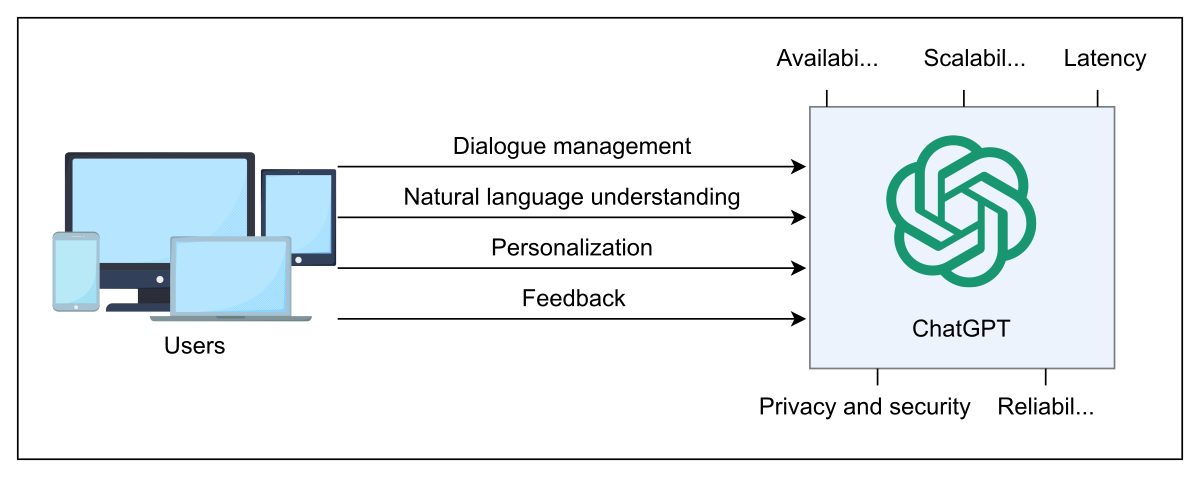
\includegraphics[width=0.5\textwidth]{Images/chapter_41/section_6392521611411456/6073177270517760.png}
 
\end{figure}

How does the system differentiate between interpreting incomplete or ambiguous user inputs?
\\
Use the AI assessment widget below to submit your solution and get an interactive response.

\textbf{Question:}

Incomplete user inputs

\textbf{Reference Answer:}

A conversational AI distinguishes incomplete or ambiguous inputs by analyzing the surrounding context and the user's previous messages. It applies intent recognition and confidence scoring to identify the most likely meaning behind unclear phrases. When confidence is low, the system may ask clarifying questions to ensure it interprets the user's intent accurately.

The next step in designing a system is to estimate the resources needed for its smooth operation. Let's discuss them in the following section:

\subsection{Resource estimation}\label{at_T27Z9YYbh6QA8Prz04}
\\
Let's break down the resource requirements for the ChatGPT system---the servers, storage, and bandwidth needed to handle a large user base. To keep our estimation practical and manageable, we'll use the following assumptions.

\begin{itemize}
\item
\protect\phantomsection\label{y-7DOcrw778t_neuN26Rz}
ChatGPT has~1 billion users, with~150 million daily active users (DAU)~interacting with the system.
\item
\protect\phantomsection\label{uVauik7xf4QhJrOju60eN}
On average, each active user sends~10 requests daily, making it 1.5 billion requests daily.
\item
\protect\phantomsection\label{u3nmgQVhSfKq0383BrSM9}
The size of each user request is approximately~(The 1 KB request size is estimated based on typical request components: metadata (200--300 bytes) for user identification and timestamps, headers (300--400 bytes) for protocol-specific routing, user input (\textasciitilde400--500 bytes) assuming an average of 250--300 characters, and additional overhead (\textasciitilde100 bytes) for security and integrity checks.)2 KBRequestSize2kb(The 1 KB request size is estimated based on typical request components: metadata (200--300 bytes) for user identification and timestamps, headers (300--400 bytes) for protocol-specific routing, user input (\textasciitilde400--500 bytes) assuming an average of 250--300 characters, and additional overhead (\textasciitilde100 bytes) for security and integrity checks.), as most inputs are short text prompts.
\item
\protect\phantomsection\label{roNjPKc0zUMu2QViI5hBN}
The average response generated by ChatGPT is~5 KB, considering that AI-generated replies are typically longer than user requests.
\end{itemize}

\subsubsection{The number of servers estimation}\label{Jw1sa16nhhHyq5arKSxpg}
\\
We assume all users are active and making requests, resulting in~150 million requests per second. We 'll use the following formula to calculate the number of servers:

\[
\text{ Servers needed at peak load} = \frac{\text{Number of requests/second}}{\text{RPS of server}}
\]

Using 64,000 as the estimated RPS a server can handle from the \href{https://www.educative.io/courses/grokking-the-system-design-interview/put-back-of-the-envelope-numbers-in-perspective}{Back-of-the-envelope calculation} section, we'll calculate the required number of servers as follows:

\[
\text{Servers\ needed\ at\ peak\ load} = \frac{150 \text{ million}}{64,000} \approx \text{ 2343 servers}
\]

\begin{figure}[htbp]
 \centering
 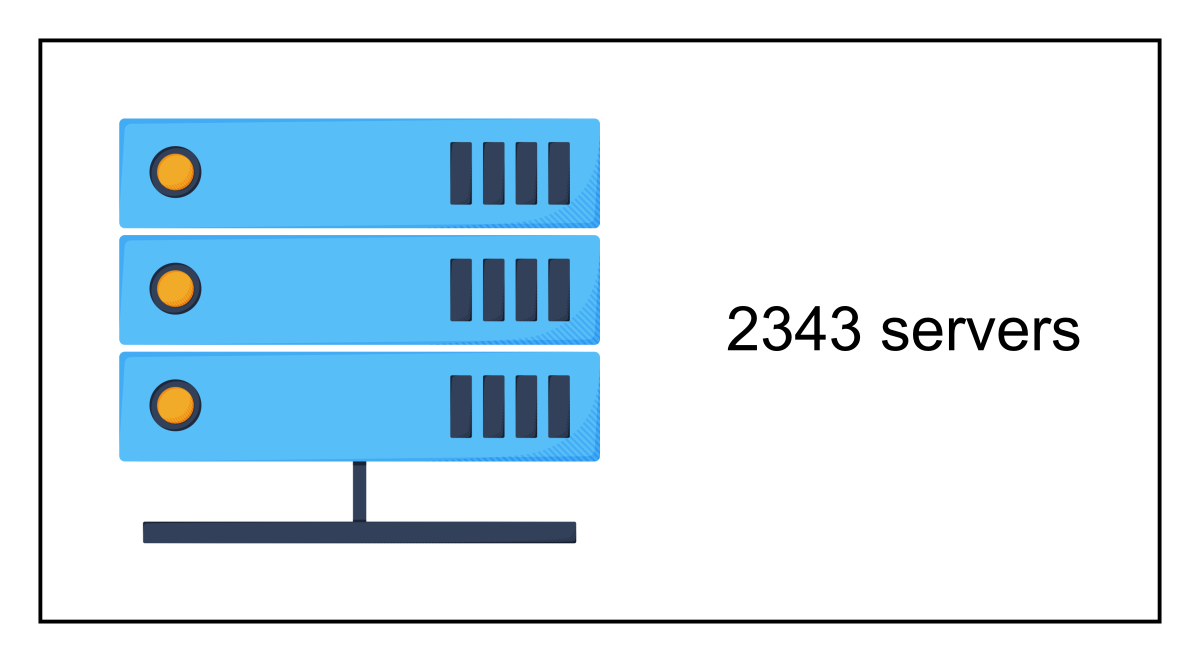
\includegraphics[width=0.15\textwidth]{Images/chapter_41/section_6392521611411456/5369486775287808.png}
 \caption{Number of servers required for ChatGPT}
\end{figure}

\begin{quote}
\textbf{Note:} We've estimated the application servers needed for the ChatGPT system, but there's more to consider. Since generative AI relies on GPU servers for fast inferences, it's crucial to factor them in. For a quick estimation of GPU requirements, check out the \href{https://www.educative.io/courses/generative-ai-system-design/back-of-the-envelope-calculations-for-the-model-training}{back-of-the-envelope calculations}.
\end{quote}
\subsubsection{Storage estimation}\label{ARB00ShfHGg7yxCcT13pi}
\\
The required storage depends on the total number of requests and their size. We'll use the following formula to compute the storage:

\[
\text{Total}_{\text{storage}} = \text{Total}_{\text{daily}\ \text{requests}}× \text{Request size}
\]

Below is a calculator to help us estimate our required resources.

\begin{quote}
\textbf{Note:} You can change the value highlighted in yellow color to see the change in storage requirement.
\end{quote}

\begin{itemize}
\tightlist
\item
Total daily request = Total DAU × average daily request per user = 150 million × 10 = 1500 million
\item
Total storage = Total daily requests × request size = 1500 × 2 KB = 3 TB
\end{itemize}

Modern deep learning models are often massive, requiring significant storage and computational power. For example, a model with 3 billion parameters in FP16 (16-bit floating point) format occupies around 6 GB(= 3 billion x 2 bytes = 6 GB) of storage. To enable real-time inference, such models are typically loaded into GPU memory, and when dealing with even larger architectures, they are distributed across multiple GPUs to balance the computational load efficiently.

\begin{figure}[htbp]
 \centering
 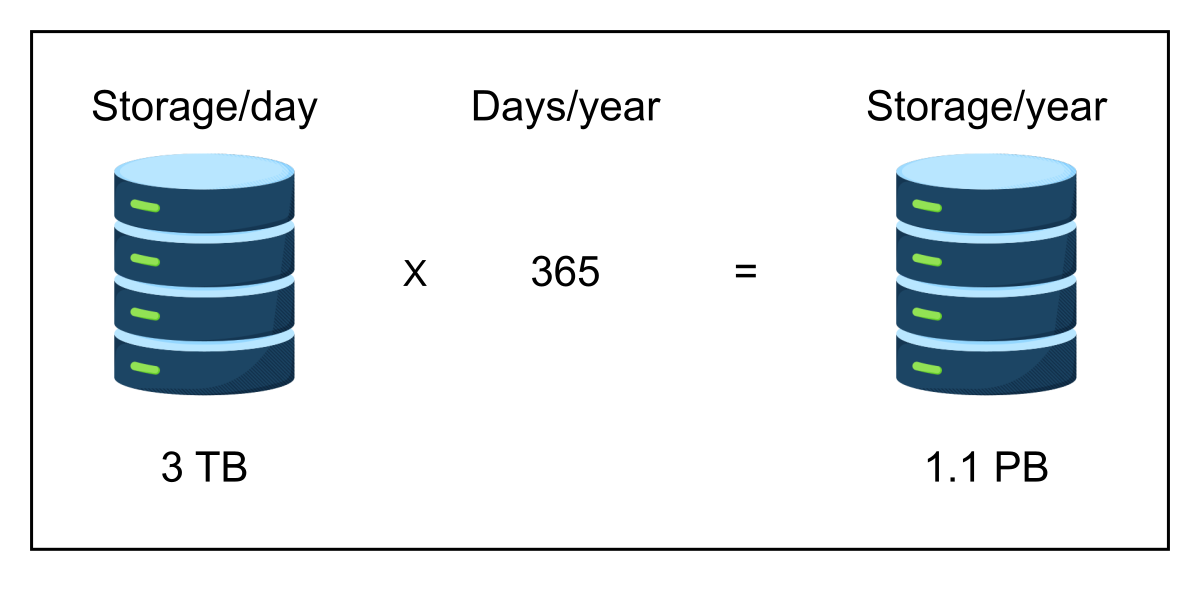
\includegraphics[width=0.5\textwidth]{Images/chapter_41/section_6392521611411456/6491617317748736.png}
 \caption{Total storage required by ChatGPT in a year}
\end{figure}

\subsubsection{Bandwidth estimation}\label{WFS5qKokXNaCrEAWi_hxO}
\\
Bandwidth estimation is essential for understanding network resource requirements and ensuring efficient data transmission. It is calculated separately for~incoming~and~outgoing~traffic, as each depends on different factors.
\\
\paragraph{Incoming bandwidth}\label{pXK3DEZTuwXPPqhUKeOcz}
\\
Incoming bandwidth is determined by the~number of incoming requests per second~and the~size of each request. Since most user requests to ChatGPT are relatively short, we assume an average request size of 2 KB, as mentioned above.
\\
The total incoming bandwidth can be calculated using the formula:

\[
\text{Total}_{\text{incoming bandwidth}} = \text{Total}_{\text{requests/sec}} \times \text{Total}_{\text{request size}}
\]


\begin{quote}
\textbf{Note:} We can adjust the values in the table to see how the incoming bandwidth varies.
\end{quote}
\\
\paragraph{Outgoing bandwidth}\label{hv8E31EYO-wGz2vDiZC3g}
\\
Outgoing bandwidth is determined by the~number of responses per second~and the~size of each response. Since ChatGPT dynamically generates responses based on user input, the response size may vary. However, for estimation purposes, we assume an average response size of 5 KB per request.
\\
The total outgoing bandwidth can be calculated using the formula:

\[
\text{Total}_{\text{outgoing bandwidth}} = \text{Total}_{\text{responses/sec}} \times \text{Total}_{\text{response size}}
\]

As user requests increase, the outgoing bandwidth consumption scales accordingly. Unlike incoming bandwidth, which is primarily influenced by short user requests, outgoing bandwidth is significantly higher due to the larger size of generated responses. We can calculate the outgoing bandwidth using the calculator given below:


\begin{quote}
\textbf{Note:} We can adjust the values in the table to see how the values change.
\end{quote}
\subsection{Building blocks we will use}\label{hGj3nJg0C6d9XFM0Ec_sS}
\\
Now that we have completed the resource estimations, let's identify the essential building blocks to design a ChatGPT system. Below are the core components:

\begin{figure}[htbp]
 \centering
 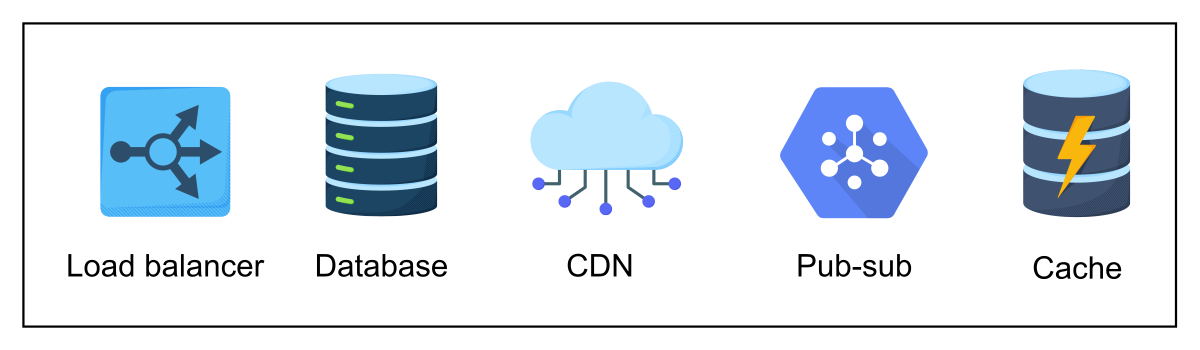
\includegraphics[width=0.5\textwidth]{Images/chapter_41/section_6392521611411456/5021893192974336.png}
 \caption{Essential building blocks required to design a ChatGPT system}
\end{figure}

\begin{enumerate}
\item
\protect\phantomsection\label{E6a8kU_iT_yE-3QySzSCD}
\href{https://www.educative.io/courses/grokking-the-system-design-interview/introduction-to-load-balancers}{\textbf{Load balancers}} distribute user requests across multiple servers and services.
\item
\protect\phantomsection\label{2vMPysixS2rdYKAUR4bDX}
\href{https://www.educative.io/courses/grokking-the-system-design-interview/introduction-to-databases}{\textbf{Databases}}~are needed to store data in a graph format and associated metadata.
\item
\protect\phantomsection\label{m__q9RBRpwLRNN2t2tXyk}
\href{https://www.educative.io/courses/grokking-the-system-design-interview/system-design-the-content-delivery-network-cdn}{\textbf{CDNs}}~deliver content to end users, reducing delay and the burden on end-servers.
\item
\protect\phantomsection\label{ZgiT0GUGNQJFPh-J1uB6K}
\href{https://www.educative.io/courses/grokking-the-system-design-interview/system-design-the-pub-sub-abstraction}{\textbf{A pub-sub system}} manages real-time messaging and events within the system.
\item
\protect\phantomsection\label{QfVhtkrrV6PmIQoVupeMk}
A \href{https://www.educative.io/courses/grokking-the-system-design-interview/system-design-the-distributed-cache}{\textbf{cache}}~is an important building block for keeping frequently accessed data.
\end{enumerate}
\\
In addition to the building blocks mentioned, other key components, such as an API gateway and ZooKeeper, play a crucial role in the system's design. We 'll discuss these in the next lesson as we dive into ChatGPT's System Design.

% End of section content